\begin{figure}[t]
\centering
% Vector drawing generated by tools/figures/build.py; rerun it after changing the figure.
\ifbilingual
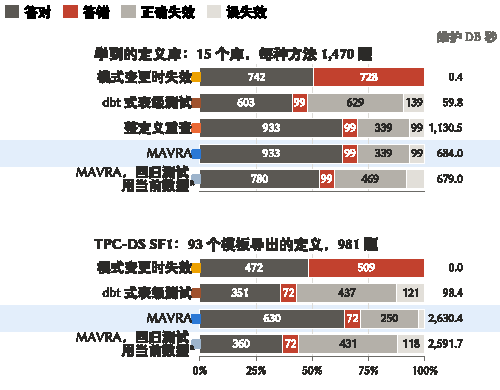
\includegraphics[width=\linewidth]{figures/replay-outcomes-zh}
\else
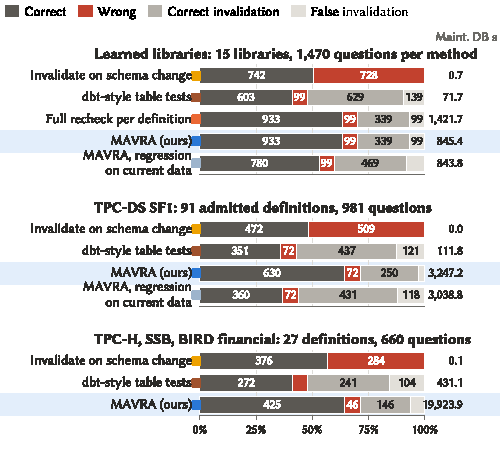
\includegraphics[width=\linewidth]{figures/replay-outcomes}
\fi
\caption{\bt{Library replay: \RpLibs\ learned libraries under \RpChanges\ data changes, \RpCondN\ scored questions per method, split by outcome; numbers at the right are maintenance database seconds. Every method uses the agent's own learning SQL for admission and as the G8 reference. Revalidation methods serve wrong answers only under the unit change, which no condition covers. $^a$Without relearning. $^b$G8 reference is the benchmark's gold SQL, which filters on the distinguishing columns in advance.}{定义库回放：\RpLibs\ 个学到的定义库，\RpChanges\ 种数据变化，每种方法 \RpCondN\ 道计分题，按结果划分；右侧数字为维护数据库秒数。所有方法都以智能体自己的学习 SQL 准入，并以它作 G8 的对照。各重验证方法只在任何条件都不覆盖的单位变化下提供错误答案。$^a$不重新学习。$^b$G8 对照为基准的标准答案 SQL，它预先带有区分列过滤。}}
\label{fig:replay}
\Description{Horizontal stacked bars, one per method, splitting 1,470 scored questions into correct, wrong, correct invalidation, and false invalidation. Schema-change invalidation answers 742 correctly and 728 wrongly; table tests 603 correct, 99 wrong, 629 correct invalidations; invalidate-on-write answers nothing; definition-level, the check-result cache, and MAVRA each answer 780 correctly and 99 wrongly with 469 correct invalidations; MAVRA with the gold SQL answers 933 correctly and 99 wrongly. Maintenance database time ranges from 0.4 s for invalidate-on-write to 1,114 s for definition-level, with MAVRA at 674 s.}
\end{figure}
